%%%%%%%%%%%%%%%%%%%%%%%%%%%%%%%%%%%%%%%%%%%%%%%%%%%%%%%%%%
%%
%% MARK: Title
%%
%%%%%%%%%%%%%%%%%%%%%%%%%%%%%%%%%%%%%%%%%%%%%%%%%%%%%%%%%%

\chapter*{\S B11. $1$-Forms on Half-Lines}
\setcounter{footnote}{0}

%%%%%%%%%%%%%%%%%%%%%%%%%%%%%%%%%%%%%%%%%%%%%%%%%%%%%%%%%%
%%
%% MARK: Abstract
%%
%%%%%%%%%%%%%%%%%%%%%%%%%%%%%%%%%%%%%%%%%%%%%%%%%%%%%%%%%%

\begin{abstract}
  In this note we characterize the differential $1$-forms
  defined on the various half-lines $\Delta$,
  $\Delta_n$, $\Delta_\infty$,
  that share the same underlying set $\LeftClosedInterval{0,\infty}$.
\end{abstract}

We consider a series of diffeologies on the set $\LeftClosedInterval{0,\infty}$:

(A) Equipped with the subset diffeology,
it is a {\em manifold with boundary} $\{0\}$, \cite[\textsection\,4.12, 4.16]{PIZ13}.
It is denoted by $\Delta$.

(B) Equipped with the pushforward of the standard diffeology of $\RR^n$,
$n>0$,
by the norm-square map:
$$
  \Sq: \RR^n \to \LeftClosedInterval{0,\infty} \quad \mbox{with} \quad \Sq : x \mapsto \Norm{x}^2,
  $$
it represents the quotients $\Delta_n = \RR^n/\O(n)$ (op.\,cit. \textsection\,1.50, Ex. 50).
We denote $\Delta_\infty=\lim_{n\to \infty}\Delta_n$,
and when we write $\Delta_n$, we allow $n$ to also represent $\infty$.

\Note{1.}
No two of the half-lines above are diffeomorphic.
We recall that $\dim_0(\Delta_n)=n$, $\dim_0(\Delta_\infty)=\infty$ and $\dim_0(\Delta)=\infty$,
(op.\,cit. Ex. 50,51) and ``A few half-lines'' in these notes.

\Note{2.}
The choice of the function $\Sq$ to characterize the quotient $\RR^n/\O(n)$ is irrelevant.
Any other bijection with the space of orbits could have been used to push forward the standard diffeology of $\RR^n$,
as explained in (op.\,cit. \textsection\,1.52).
For example we could have chosen equivalently $X \mapsto \Norm{X}$,
but then the injection $j:\LeftClosedInterval{0,\infty} \to \RR$ would not have been smooth.

%%%%%%%%%%%%%%%%%%%%%%%%%%%%%%%%%%%%%%%%%%%%%%%%%%%%%%%%%%
%%
%% MARK: 1-forms on the half-lines
%%
%%%%%%%%%%%%%%%%%%%%%%%%%%%%%%%%%%%%%%%%%%%%%%%%%%%%%%%%%%

%\section{$1$-Forms on the half-lines}\n

\begin{Article}{The $1$-forms are closed.}{}
  Every differential $1$-form defined on $\Delta_n$,
  $\Delta_\infty$,
  or $\Delta \subset \RR$,
  is closed.
  Moreover,
  every half-line is contractible.
  Therefore,
  every $1$-form is exact.
  
  \Note In the case $n=1$,
  the $1$-forms are closed simply because the dimension of $\Delta_1$ is $1$ (op.\,cit. \textsection\,6.39).
  But because the dimensions of $\Delta_n$ for $n>1$ and $\Delta$ at the origin are $n$ or $\infty$,
  the dimension argument does not apply so simply.
\end{Article}

\begin{proof}
  Any of these half-lines has $\LeftClosedInterval{0,\infty}$ as underlying space,
  only the diffeology changes.
  In each case,
  the subset $\OpenInterval{0,\infty}$ is D-open.
  In each case,
  the diffeology induced on $\OpenInterval{0,\infty}$ is the standard diffeology.
  The difference in behavior of the diffeology occurs only in a neighborhood of $\{0\}$.
  
  Now,
  let $\alpha$ be a $1$-form on a half-line,
  let $P$ be an $m$-plot and $U \subset \RR^m$ be its domain.
  The subset $V = P^{-1}(\OpenInterval{0,\infty})$ is open in $U$ and because $\OpenInterval{0,\infty}$ is $1$-dimensional, $d[\alpha(P\restriction V)]=0$.
  The complement $W$ of $V$ in $U$ is closed. On its interior $\mathring{W}$ the plot is constant,
  therefore $\alpha(P\restriction \mathring{W})= 0$,
  and then $d[\alpha(P\restriction \mathring{W})]= 0$.
  
  Now,
  on the boundary $\partial V = \bar V - V = W - \mathring{W}$,
  every point $r$ is a limit $\lim_{n\to\infty} r_n$, with $r_n \in V$.
  Thus,
  by continuity,
  for all $\xi, \xi' \in \RR^m$,
  $d[\alpha(P)]_r(\xi, \xi') = \lim_{n\to\infty} d[\alpha(P\restriction V)]_{r_n}(\xi, \xi') = 0$.
  Hence,
  $d\alpha(P) = 0$ everywhere,
  that is,
  $d\alpha=0$.
  
  Next,
  about contractibility.
  Since the radial retraction $x \mapsto sx$ in $\RR^n$ is equivariant under the action of $\O(n)$,
  the quotients $\Delta_n=\RR^n/\O(n)$ are contractible,
  and also the limit $\Delta_\infty$.
  For $\Delta$ we have the retraction $\rho_s : t \mapsto s^2t$.
  The map $(s,t) \mapsto s^2t$, defined on $\RR\times\Delta$, takes its values in $\Delta$ and is smooth.
  Thus,
  $\Delta$ is contractible.
  According to (op.\,cit. \textsection\,6.90) every closed differential form on a contractible diffeological space is exact.
  Therefore,
  every $1$-form on these half-lines is the differential of a smooth function;
  this function can be normalized to vanish at the origin,
  and then is unique.
\end{proof}

\begin{Article}{The case of $\Delta$.}{}
  Every differential $1$-form on the embedded half-line $\Delta \subset \RR$ is the restriction of a differential $1$-form defined on $\RR$.
  In other words,
  the natural induction $j : \LeftClosedInterval{0,\infty} \to \RR$ induces a surjective pullback $j^* : \DForms^1(\RR) \to \DForms^1(\Delta)$.
  That is, for every $\alpha \in \DForms^1(\Delta)$,
  there exists $a\in \Cinfty(\RR,\RR)$ such that $\alpha_x=a(x)\, dx$, for all $x\geq 0$.
\end{Article}

\begin{proof}
  Thanks to (op.\,cit. \textsection\,4.13) we know that a smooth function from $\Delta$ to $\RR$ is the restriction of a smooth function from $\RR$ to $\RR$.
  Together with the proposition above, this gives the result.
\end{proof}

\begin{Article}{The case of $\Delta_n$.}{}
  The set $\LeftClosedInterval{0,\infty}$ is equipped with the pushforward of the standard diffeology of $\RR^n$
  by the norm-square map $\Sq$.
  This identifies $\Delta_n$ with $\RR^n/\O(n)$ via $\Class(X) \simeq \Norm{X}^2$.
  The injection $j:\Delta_n \simeq \LeftClosedInterval{0,\infty} \to \RR$ is smooth.
  The pullback $j^* : \DForms^1(\RR) \to \DForms^1(\Delta_n)$ is, here again,
  surjective.%
  \footnote{Note that the inclusion $j$ is smooth and injective but not an induction.}
\end{Article}

\begin{proof}
  The smoothness of the injection follows from the smoothness of the square map $\Sq:\RR^n \to \LeftClosedInterval{0,\infty}$, with $\Sq(X)=\Norm{X}^2$.
  
  Now,
  for the same reason as before, every $1$-form $\alpha$ on $\Delta_n$ is exact,
  that is,
  there exists a function $f\in \Cinfty(\Delta_n,\RR)$ such that $\alpha = df$.
  Pulled back to $\RR^n$,
  we have $\Sq^*(\alpha) = \Sq^*(df) = d(f\circ \Sq)$.
  The function $F=f\circ\Sq$ is smooth and invariant under $\O(n)$.
  Conversely, every smooth function $F : \RR^n \to \RR$ that is $\O(n)$-invariant is the pullback,
  by $\Sq$,
  of a smooth function $f$ on $\Delta_n$.
  Thus, every $1$-form on $\Delta_n$ is the pushforward of a differential $dF$,
  where $F$ is smooth and $\O(n)$-invariant.
  
  Let us restrict $F$ to the subspace of vectors $(x,0,\ldots,0)$, $x\in \RR$,
  and denote $F(x)$ for $F(x,0,\ldots,0)$.
  We have $F(x)= f(x^2)$,
  that is,
  $F(x) = F(-x)$.
  By Whitney's theorem \cite{Whi43},
  there exists a smooth function $g\in \Cinfty(\RR,\RR)$ such that $F(x)=g(x^2)$.
  Thus,
  $f(x^2)=g(x^2)$,
  in other words:
  $f=g\restriction \LeftClosedInterval{0,\infty}$,
  $f$ is the restriction of a smooth function to the interval $\LeftClosedInterval{0,\infty}$.
  Hence $\alpha = df = d(g\circ j)= j^*(dg)$;
  written differently,
  $\alpha_t = a(t)\, dt$, for all $t\in \LeftClosedInterval{0,\infty}$, with $a = g'$.
  
  On $\RR^n$,
  the pullback of $\alpha$ becomes,
  $$
    \Sq^*(\alpha)_X = 2 a\big(\Norm{X}^2\big) X \cdot dX = 2 a\big(\Norm{X}^2\big) \sum_{i=1}^n X^i dX^i,
    $$
  where $a$ is a smooth function on $\RR$.
\end{proof}

\begin{Article}{The $1$-forms vanish at the origin.}{}
  Every differential $1$-form $\alpha$,
  defined on any half-line $\Delta$ or $\Delta_n$ or $\Delta_\infty$,
  vanishes at the origin (op.\,cit. \textsection\,6.40).
  That is,
  for every $1$-plot $\gamma$ pointed at the origin,
  with $\gamma(0)=0$,
  we have $\alpha(\gamma)_0 = 0$.
  
  In other words, the \textit{cotangent space} reduces to $\{0\}$ at the origin (op.\,cit. \textsection\,6.48);
  it is equal to $\RR$ everywhere else.
  An interesting question would be to describe the diffeology of the cotangent space,
  and to study its parasymplectic structure,%
  \footnote{Terminology introduced in ``Example of Singular Reduction in Symplectic Diffeology''.}
  that is,
  the structure defined by the differential of its Liouville form (op.\,cit. \textsection\,6.49).
\end{Article}

\begin{proof}
  According to what precedes,
  in every case the injection $j$ from the half-line into $\RR$ is smooth,
  and the form $\alpha$ is the pullback,
  by $j$,
  of some smooth $1$-form $A\in\DForms^1(\RR)$.
  Thus, $\alpha(\gamma)_0 = j^*(A)(\gamma)_0 = A(j \circ\gamma)_0$.
  But $j \circ\gamma(0)=0$ and $j \circ\gamma(t)\geq 0$ imply that $\frac{d}{dt}(j\circ\gamma)(0) = 0$.
  Therefore, $A(j \circ\gamma)_0 = A_0\left(\frac{d}{dt}(j\circ\gamma)(0)\right)=0$, and $\alpha(\gamma)_0=0$.
\end{proof}

\begin{Article}{The $1$-forms as a $1$-dimensional module.}{}
  From what precedes we conclude that,
  in every case:
  $\Delta_\star = \Delta$ or $\Delta_n$ or $\Delta_\infty$,
  the space of differential $1$-forms $\DForms^1(\Delta_\star)$ is a $1$-dimensional module over $\DForms^0(\Delta_\star)$,
  with $dt\restriction \LeftClosedInterval{0,\infty}$ as a generator.
\end{Article}

\begin{Article}{Gauges on diffeological spaces.}{}
  There is a notion of volume for diffeological spaces of finite constant dimension
  in (op.\,cit. \textsection\,6.44) that almost applies to the half-lines but not completely.
  First of all,
  in our case the dimension is not constant (except for $n=1$),
  but more importantly,
  the $1$-form vanishes at the origin,
  whereas volumes are assumed to be nowhere vanishing.
  Nevertheless,
  in every case above,
  the space of $1$-forms is a $1$-dimensional module over the space of smooth functions,
  and this is an important observation.
  This leads to the introduction of the concept of {\em $k$-gauge} on a diffeological space,
  which is slightly different from the concept of volume, but pursues the same idea:
  
  \textbf{Definition.}
  We call a {\em $k$-gauge} on a diffeological space $X$
  any $k$-form generating $\DForms^k(X)$ as a $1$-dimensional module over $\DForms^0(X)$.
  
  \smallskip In our case, for every half-line $X$,
  the pullback $j^*(dt)$,
  where $j$ is the smooth injection of $\LeftClosedInterval{0,\infty}$ into $\RR$,
  is a generator of $\DForms^1(X)$.
  The concept of $k$-gauge on diffeological spaces is worth studying.
  There are several questions around it that need to be answered.
\end{Article}

\vfill
\centerline{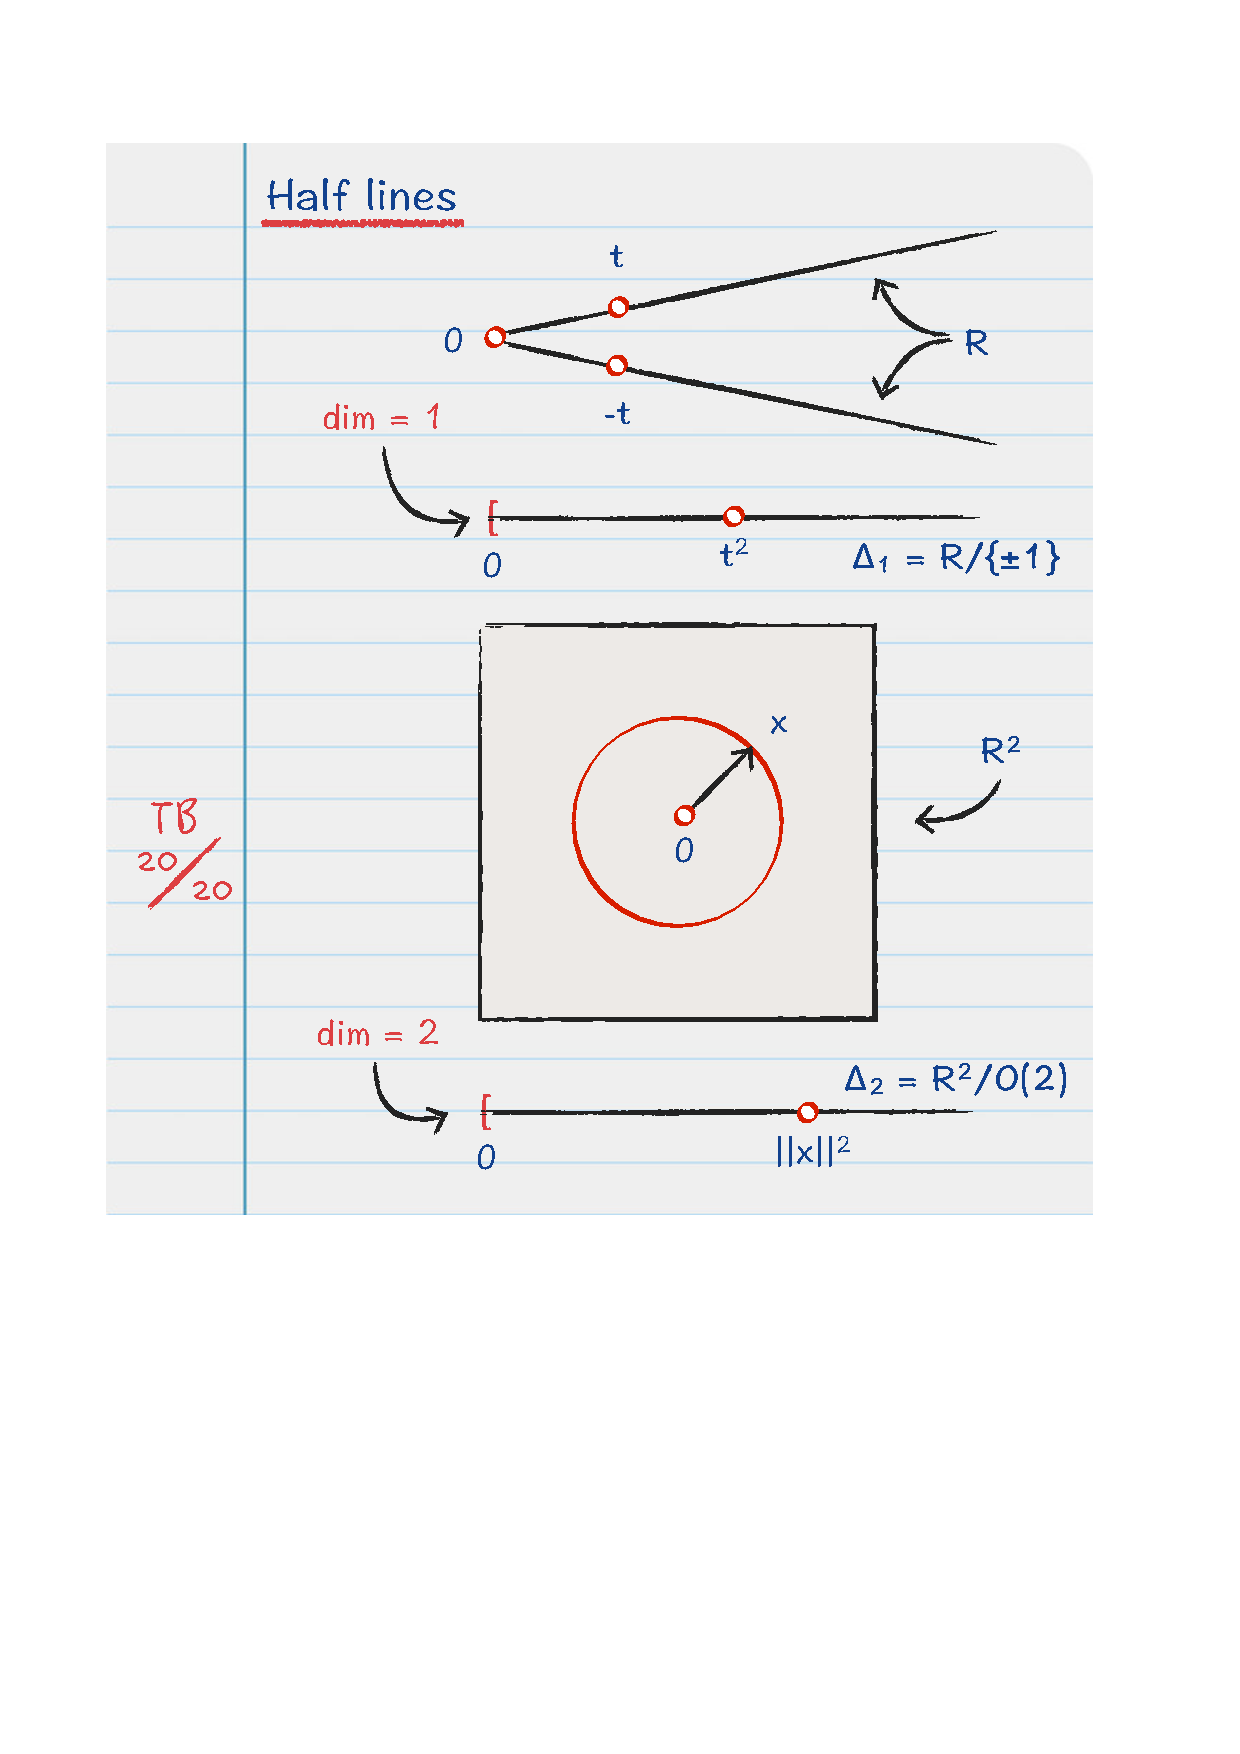
\includegraphics[width=.9\textwidth]{Figures/Half-lines.pdf}}
\vfill
